\section{Cài đặt công cụ}

Công cụ phân tích mã nguồn Rust được phát triển từ mã nguồn của công cụ Joern.
Công cụ được cài đặt bằng ngôn ngữ Rust và Scala. Kiến trúc tổng quan của công cụ được
mô tả ở Hình 4.1

\begin{figure}[H]
	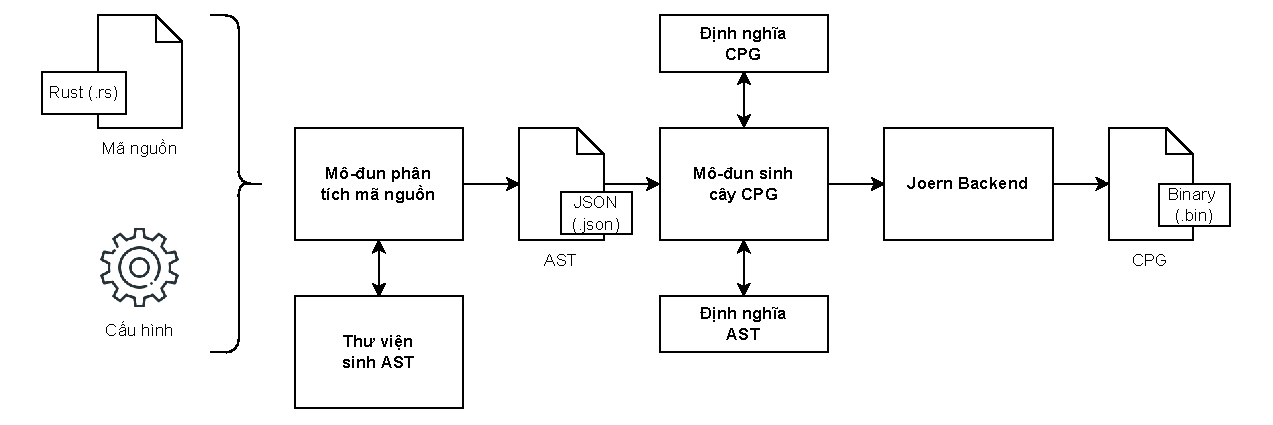
\includegraphics[width=1\columnwidth]{figures/c4/c4_install_flow.drawio.pdf}
	\centering
	\caption{Kiến trúc công cụ.}
	\label{img:c4_install_flow}
\end{figure}

Công cụ gồm hai mô-đun là $Rust\ Parser$ và $Joern$ trong đó $Joern$ là mô-đun
chính. Mô-đun GoParse được cài đặt bằng ngôn ngữ Rust. Mô-đun này sẽ nhận đầu vào là
đường dẫn đến thư mục dự án chứa mã nguồn Rust và thực hiện việc phân tích mã nguồn
thành cây cú pháp mã nguồn, xử lý kiểu dữ liệu và lưu cây cú pháp mã nguồn vào các
tệp JSON. $Joern$ được cài đặt bằng ngôn ngữ Scala và được phát triển từ mã nguồn
của công cụ $Joern$. Mô-đun thực hiện nhận mã nguồn đầu vào, gọi mô-đun $Rust\ Parser$ để
dựng cây cú pháp mã nguồn và sau đó xây dựng đồ thị thuộc tính mã nguồn từ các thông
tin trong cây cú pháp mã nguồn. Đầu ra của mô-đun này cũng là đồ thị thuộc tính mã
nguồn được lưu dưới dạng tệp nhị phân (.bin). Đây cũng là đầu ra của cả công cụ. Chúng
ta có thể dùng một số công cụ được $Joern$ cung cấp sẵn để thao tác với đồ thị này như xuất đồ thị dưới nhiều định dạng khác nhau như neo4jcsv, graphml, graphson, dot bằng
công cụ $Joern\ Export$, thực hiện các câu lệnh truy vấn trên đồ thị hoặc quét đồ thị để tìm
lỗ hổng trong mã nguồn bằng công cụ $Joern\ Scan$.

\subsection{Mô-đun xây dựng cây cú pháp trừu tượng Rust Parser}

Chức năng chính của $Rust\ Parser$ là nhận thông tin đường dẫn đến mã nguồn, lọc các
tệp mã nguồn Rust, sinh cây cú pháp trừu tượng, xử lý kiểu dữ liệu cho các nút định danh
(identifier) và lưu kết quả vào các tệp JSON. Các thành phần trong mô-đun này bao gồm
cli, parser, resolver, ast và util. Chức năng chi tiết của từng thành phần được mô tả như
sau:

\begin{itemize}
\item Thành phần cli làm nhiệm vụ xử lý và cung cấp giao diện dòng lệnh (CLI), nhận
đầu vào là đường dẫn đến dự án Rust, nhận các cấu hình (ví dụ như đường dẫn lưu
các tệp đầu ra hoặc danh sách các tệp mã nguồn cần bỏ qua) và gọi các chức năng
phân tích.
\item Thành phần parser thực hiện nhận thông tin từ thành phần cli, từ đó đọc các tệp mã
nguồn của Rust có đuôi là ".rs" từ dự án đầu vào, phân tích các tệp tin này và sinh
cây cú pháp trừu tượng.
\item Thành phần resolver cung cấp các API phục vụ việc xử lý kiểu dữ liệu.
\item Thành phần ast chứa các cấu trúc định nghĩa các loại nút và thuộc tính của từng
loại nút của cây cú pháp trừu tượng.
\item Thành phần util cung cấp các tiện ích chung bao gồm xử lý tệp tin và xử lý nhật ký
(log).
\end{itemize}
Hình 4.2 biểu diễn các thành phần của mô-đun $Rust\ Parser$, các mũi tên biểu mối
quan hệ sử dụng giữa các thành phần này.

\subsection{Mô-đun xây dựng đồ thị thuộc tính mã nguồn Joern}

Mô-đun $Joern$ thực hiện nhiệm vụ xây dựng đồ thị thuộc tính mã nguồn (CPG)
từ cây cú pháp trừu tượng AST. Mô-đun sẽ thực hiện đọc thông tin từ các tệp JSON được
tạo ra từ mô-đun $Rust\ Parser$ và xây dựng đồ thị thuộc tính mã nguồn (CPG). Mô-đun này
được phát triển từ mô-đun $Joern$ của công cụ $Joern$ nên sử dụng lại một số thành
phần có sẵn của $Joern$ bao gồm các thành phần console, semanticcpg, codepropertygraph
và x2cpg. Dưới đây tôi sẽ mô tả chức năng của từng thành phần:
\begin{itemize}
\item Thành phần console thực hiện chức năng tương tự như thành phần cli của mô-đun
$Rust\ Parser$.
\item Thành phần rust-language-frontend đảm nhận nhiệm vụ nhận đường dẫn đến mã nguồn từ thành phần console, gọi mô-đun $Rust\ Parser$ để sinh cây cú pháp trừu tượng sau đó đọc các tệp JSON được sinh ra và xây dựng thành đồ thị thuộc tính mã nguồn.
\item Thành phần codepropertygraph chứa các lớp định nghĩa các đỉnh và cạnh của đồ thị thuộc tính mã nguồn.
\item Thành phần x2cpg cung cấp các tiện ích để ánh xạ các thuộc tính từ các nút của cây cú pháp trừu tượng sang thuộc tính của các đỉnh trong đồ thị thuộc tính mã nguồn.
\item Thành phần semanticcpg chứa các tiện ích cho phép vấn đồ thị thuộc tính mã nguồn. Thành phần này được sử để thực hiện các tác vụ hậu xử lý sau khi đồ thị thuộc tính mã nguồn được xây dựng (ví dụ như bổ sung thông tin hoặc tạo các đỉnh liên kết).
\end{itemize}

Hình 4.3 biểu diễn các thành phần của mô-đun $Rust\ Parser$, các mũi tên biểu mối
quan hệ sử dụng giữa các thành phần này.

